\tikzset{
   plane/.pic = {
    \draw[fill]  plot[smooth, tension=0.6] coordinates {
        (-0.65,-0.9) 
        (-0.6,-0.85) 
        (-0.4,-0.75) 
        (-0.25,-0.65) 
        (-0.15,-0.5) 
        (-0.12,-0.3) 
        (-0.1,-0.1) 
        (0,0) 
        (0.1,-0.1) 
        (0.12,-0.3) 
        (0.15,-0.5) 
        (0.25,-0.65) 
        (0.4,-0.75) 
        (0.6,-0.85) 
        (0.65,-0.9)
        } -- plot[smooth, tension=0.6] coordinates {
        (0.65,-0.9) 
        (0.15,-0.91)
        (0.35,-1.1) 
        (0.37,-1.15)
        } -- plot[smooth, tension=0.6] coordinates {
        (0.37,-1.15)
        (0,-1.12) 
        (-0.37,-1.15) 
        } -- plot[smooth, tension=0.6] coordinates {
        (-0.37,-1.15)
        (-0.35,-1.1) 
        (-0.15,-0.91) 
        (-0.65,-0.9) 
        } -- cycle;
   }
}
\newcommand{\rvec}[1]{\ensuremath{{\boldsymbol{\underline{#1}}}}}
\newcommand{\rv}[1]{\ensuremath{{\boldsymbol{#1}}}}
\newcommand{\mat}[1]{{\ensuremath{{\mathbf{#1}}}}}

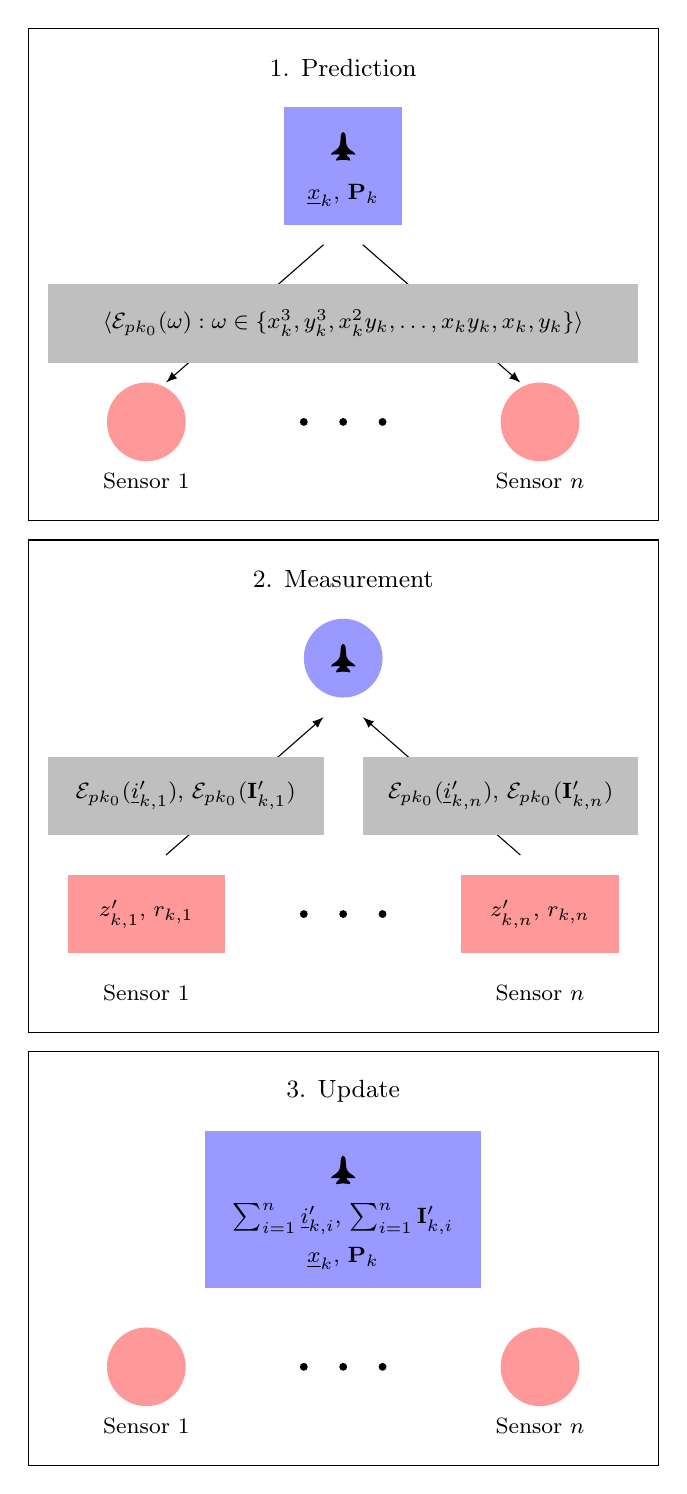
\begin{tikzpicture}[font=\footnotesize]


    % Prediction
    \draw  (0,1.75) rectangle (8,8);
    \node at (4,7.5) {\small 1. Prediction};

    % Navigator
    \fill  [blue!40] (3.25,7) rectangle (4.75,5.5);
    \pic[xscale=0.22,yscale=0.3] at (4,6.6725) {plane};
    \node at (4,5.875) {$\rvec{x}_k$, $\mat{P}_k$};
    
    % Sensors
    \fill  (1.5,3) [red!40] ellipse (0.5 and 0.5);
    \node at (1.5,2.25) {Sensor $1$};
    \fill  (6.5,3) [red!40] ellipse (0.5 and 0.5);
    \node at (6.5,2.25) {Sensor $n$};
        
    \fill [black] (3.5,3) circle (0.05);
    \fill [black] (4,3) circle (0.05);
    \fill [black] (4.5,3) circle (0.05);
        
    % Arrows
    \draw [-latex] plot[smooth, tension=.7] coordinates {(3.75,5.25) (1.75,3.5)};
    \draw [-latex] plot[smooth, tension=.7] coordinates {(4.25,5.25) (6.25,3.5)};
    
    \fill [lightgray]  (0.25,4.75) rectangle (7.75,3.75);
    \node at (4,4.25) {$\langle\mathcal{E}_{pk_0}(\rv{\omega}): \rv{\omega} \in \{\rv{x}^3_k, \rv{y}^3_k, \rv{x}^2_k\rv{y}_k, \dots , \rv{x}_k\rv{y}_k, \rv{x}_k, \rv{y}_k\}\rangle$};
    
    
    % Measurement
    \draw  (0,-4.75) rectangle (8,1.5);
    \node at (4,1) {\small 2. Measurement};
    
    % Navigator
    \fill  (4,0) [blue!40] ellipse (0.5 and 0.5);
    \pic[xscale=0.22,yscale=0.3] at (4,0.1725) {plane};
        
    % Sensors
    \fill  [red!40] (7.5,-3.75)  rectangle (5.5,-2.75);
    \node at (1.5,-4.25) {Sensor $1$};
    \fill  [red!40] (2.5,-3.75)  rectangle (0.5,-2.75);
    \node at (6.5,-4.25) {Sensor $n$};
    
    \node at (1.5,-3.25) {$\rv{z}'_{k,1}$, $\rv{r}_{k,1}$};
    \node at (6.5,-3.25) {$\rv{z}'_{k,n}$, $\rv{r}_{k,n}$};
    
    \fill [black] (3.5,-3.25) circle (0.05);
    \fill [black] (4,-3.25) circle (0.05);
    \fill [black] (4.5,-3.25) circle (0.05);
    
    % Arrows
    \draw [-latex] plot[smooth, tension=.7] coordinates {(1.75,-2.5) (3.75,-0.75)};
    \draw [-latex] plot[smooth, tension=.7] coordinates {(6.25,-2.5) (4.25,-0.75)};
    
    \fill [lightgray]  (0.25,-1.25) rectangle (3.75,-2.25);
    \node at (2,-1.75) {$\mathcal{E}_{pk_0}(\rvec{i}'_{k,1})$, $\mathcal{E}_{pk_0}(\mat{I}'_{k,1})$};
    \fill [lightgray]  (4.25,-1.25) rectangle (7.75,-2.25);
    \node at (6,-1.75) {$\mathcal{E}_{pk_0}(\rvec{i}'_{k,n})$, $\mathcal{E}_{pk_0}(\mat{I}'_{k,n})$};
    
    
    % Update
    \draw  (0,-10.25) rectangle (8,-5);
    \node at (4,-5.5) {\small 3. Update};
    
    % Navigator
    \fill  [blue!40] (2.25,-6) rectangle (5.75,-8);
    \pic[xscale=0.22,yscale=0.3] at (4,-6.3275) {plane};
    \node at (4,-7.125) {$\sum_{i=1}^n \rvec{i}'_{k,i}$, $\sum_{i=1}^n\mat{I}'_{k,i}$};
    \node at (4,-7.625) {$\rvec{x}_k$, $\mat{P}_k$};
    
    % Sensors
    \fill  (6.5,-9) [red!40] ellipse (0.5 and 0.5);
    \node at (1.5,-9.75) {Sensor $1$};
    \fill  (1.5,-9) [red!40] ellipse (0.5 and 0.5);
    \node at (6.5,-9.75) {Sensor $n$};
    
    \fill [black] (3.5,-9) circle (0.05);
    \fill [black] (4,-9) circle (0.05);
    \fill [black] (4.5,-9) circle (0.05);
    
    
\end{tikzpicture}










